%!TEX TS-program = lualatex
%!TEX encoding = UTF-8 Unicode

%\frame[plain]{ % When including a large figure or table, you don't want to have the bottom and the top of the slides.
%\frame[shrink]{ % If you want to include lots of text on a slide, use the shrink option.

\begin{frame}
    
    \frametitle{But wait...}
    
    \makebox[\linewidth]{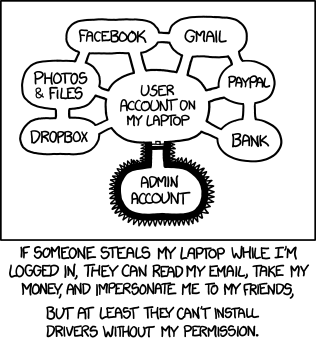
\includegraphics[width=0.5\paperwidth]{frames/img/xkcd_1200_authorization}}
    
    \small{https://xkcd.com/1200/}
    \note{
        \begin{itemize}
            \item You could say I lied. 
            \item Of course without further isolation of the filesystem process in user space it will have access to anything in user space of the user it runs on.
        \end{itemize}
    }
\end{frame}